\chapter{Engineering method}

\todo{Add more filler here}

\section{Modularity}

As mentioned previously, modularity, or a modular application, is an application
which can be extended by other pieces of software. This extensibility is useful
as features that the original developers of the application did not think about,
can be added. If this module architecture is well-designed, then this extension
can be added without changing the core application. This way of designing
software can be taken to the extreme, a zero-core application, where the only
functionality the application provides, is a way to extend the core functionality
with modules.

\subsection{How to extend an application}

There are different methods an application can be extended. The most popular one
\todo{Sauce???} uses so-called \textit{live-reload}, in which, if a module
drastic changes the functionality of an application, the application has to be
restarted, or if it is a \textit{minor} change, the module is simply loaded.
This method is extending of the application during runtime, which is the method
most commonly accepted. Another method would be \textit{compile-time-extension},
in which modules are added before the application itself is compiled. There are
some advantages and disadvantage in both approaches.

As an example, a standard user of a zero-core application will expect the
application to come bundled with all the needed functionality. This is best
achieved with the \textit{compile-time-extension} method, since the application
can be installed with the expected modules.

\subsection{Granularity}

When designing modules, the \textit{granularity} of the combined modules has to
be considered. As an example, if one where to extend the zero-core application
with the needed functionality for it to be considered an \gls{ide}, this could be
achieved by creating a singular module which does all the work. However, this
is not a modular approach, as if one wants to change some specific feature in
the \gls{ide}-module, one would have to re-create the whole module with that
specific feature implemented. Instead, if this functionality was granular,
that is to say, split into several modules, that together enable the needed
features, then it would be \textit{simpler} to modify the needed modules to
achieve the wanted feature.

\subsection{Module Family}

\begin{figure}
  \centering
  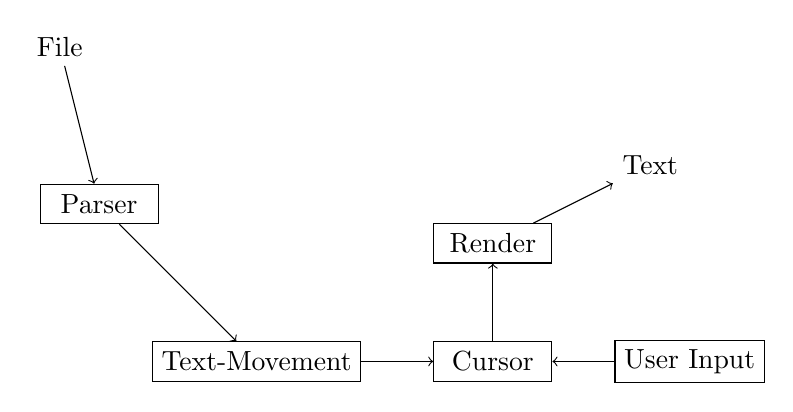
\begin{tikzpicture}
  % Nodes
  \node (file) [] at (-6, 3) {File};
  \node (parser) [rectangle, draw, minimum height=0.5cm, minimum width=1.5cm] at (-5.5, 1) {Parser};
  \node (text-movement) [rectangle, draw, minimum height=0.5cm, minimum width=1.5cm] at (-3.5, -1) {Text-Movement};
  \node (cursor) [rectangle, draw, minimum height=0.5cm, minimum width=1.5cm] at (-0.5, -1) {Cursor};
  \node (user-input) [rectangle, draw, minimum height=0.5cm, minimum width=1.5cm] at (2, -1) {User Input};
  \node (render) [rectangle, draw, minimum height=0.5cm, minimum width=1.5cm] at (-0.5, 0.5) {Render};
  \node (text) at (1.5, 1.5) {Text};
  % Arrow
  \draw[->] (file) -- (parser) node[midway, above] {};
  \draw[->] (parser) -- (text-movement) node[midway, above] {};
  \draw[<-] (cursor) -- (text-movement) node[midway, above] {};
  \draw[<-] (cursor) -- (user-input) node[midway, above] {};
  \draw[->] (cursor) -- (render) node[midway, above] {};
  \draw[->] (render) -- (text) node[midway, above] {};
\end{tikzpicture}

  \caption{Text Editor Module Family}
  \label{fig:textEditorSimple}
\end{figure}

In figure \ref{fig:textEditorSimple}, an input file is parsed to some structure
which is used to translate user actions, into cursor movements. The cursor being
the place in the file where text is written to by the user.

This is a feature that naturally shows up in a \textit{true} modular system. If
several modules together enable some feature, then those modules can be treated
as a singular module by an external module developer, depending on what they
want to extend.

\subsection{Module V.1}

We did not attempt at first, to create a zero core application; this was a
\textit{natural} conclusion to the existing problem. The first attempt was a
simple generic \gls{ide}, in which the module architecture was a concern from
day one of development. The general plan was this:

\begin{enumerate}
  \item Create an \gls{ide}
  \item Extend the \gls{ide}, to allow for a module architecture
  \item Modules call the application using some DSL
\end{enumerate}

This was the more straight forward way to work, because as we could model it of
existing \gls{ide}s, like \textit{Visual Studio Code} or \textit{Eclipse}.
Another advantage is that when implementing the application, one necessarily
gets a better understand of how eventual modules should extend the application.
This approach did unfortunately not lead to a truly modular application. Similar
issues to existing \gls{ide}s, how does one allow for \textit{everything}?
Furthermore, anything created this way, would be subpar to existing software,
which would lead to the next maintainer having to fix the core application. This
in turn, would add a lot of complexity, which the maintainers would have to deal with.

\subsubsection{Tech Stack}

Started with Rust, because a \textit{low-level} language was assumed to be
necessary, to facilitate ease of C integration, which would allow for an
extendable application, which was language agnostic.

Furthermore, using Rust in this low-level environment, gives the added advantage
of the compiler knowing then a value is unused, and automatically
\textit{de-allocating} this memory. This helps avoid memory leakage. Further
safety can be encoding in Rust robust type system, avoiding dangling pointers
and null references.

Framework we chose was Tauri, UI components can be created using JavaScript. This
framework gives a lot of security which is needed in an application which runs
third party code.
\todo{Expand upon the security aspect}

As mentioned, the UI of the application is rendered using \gls{html} and
JavaScript, making development of the UI similar to standard web development.
This enabled a low development time of UI components, since this is something
that a lot of UI and UX designers have looked into. So existing code for this
already exists and can be used.

Since any JavaScript frontend framework could be used, React was chosen, one of
the reason for this choice was due to its popularity, which again, would speed
up the development time of the application, but also due to the way React
renders. Between two different re-renders of the application, React can check
the difference between the \gls{vdom}, which is React's representation of the
\gls{dom}. It then only changes what is needed in the \gls{dom}, instead of
re-creating the entire \gls{dom}, which makes the render time quick.

\todo{Rewrite this to better connect to the previous section}
Communication between the Rust and JavaScript parts is JSON-RPC, which,
effectively, is the same as a client-server

Allows for modules in two different languages, with little effort. One that
targets the JavaScript environment, and one that targets Rust, with the
possibility to create bindings from Rust to C, enabling a whole sleuth of other
languages to be used.

This also allows for usage of existing JavaScript libraries, which can be used
with the \gls{npm}. In the \gls{npm} registry, there are around
\textit{34 million} libraries, all of which are usable in this architecture. If
the functionality that these libraries are useful for the application, is
another question. This functionality allows for quick development time for
modules, which means features that are standard in \gls{ide} can be quickly and
easily added. A concrete example of this, is the text editor. A text editor in
itself is quite complex, especially if one needs the added functionality of
\gls{lsp} support. This can be solved quite easily by adding the
\textit{Monaco} library, which is the VS Code text editor, with integrated
\gls{lsp} client support.

While this is not the best approach to implementing a text editor, a more
modular approach, by turning the text editor into a module family would be more
effective, it is good enough as a stop-gap.

\subsection{Module V.2}

\todo{Mention JS-MS and RS-MS}
\todo{Mention the backend-frontend that was introduced in this plan}
\todo{Mention the troubles with backend-frontend state coalescing.}

After 7–8 months of working on this, everything was scrapped for this new plan:

\todo{Add footnote}
\begin{enumerate}
  \item Everything* is a module
\end{enumerate}

\subsection{Elm-Architecture}

An inspiration for the new module architecture is Elm-Lang. Elm is a functional
language, aimed at frontend web development, but its architecture is quite
\todo{Maybe add some Elm-lang papers? Should probably read some}
interesting. As one can see in figure \ref{fig:elmArchitecture}, is used by some
runtime, which translates the Elm code into \gls{dom} manipulations, and translates
\gls{dom} events into \textit{Msg} which is handled by the Elm code. This was the
inspiration for the new module architecture. A module is managed by the runtime,
which is the \textit{core} application. But with some inspiration from
\gls{mvc}, where instead of the module keeping its own state, this is again
managed by the core, allowing for multiple modules to read and react to states
updated by other modules, allowing for more interactivity between modules, and
therefore being more modular.

\todo{Add source: guide.elm-lang.org/effects/}
\begin{figure}
  \centering
  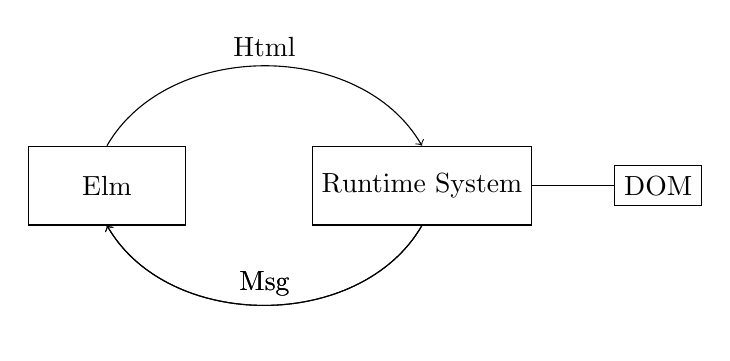
\begin{tikzpicture}
  % Nodes
  \node (p) [rectangle, draw, minimum height=1cm, minimum width=2cm] at (0, 0) {Elm};
  \node (i) [rectangle, draw, minimum height=1cm, minimum width=2cm] at (4, 0) {Runtime System};
  \node (d) [rectangle, draw, minimum height=0.5cm, minimum width=1cm] at (7, 0) {DOM};
  % Arrow
  \draw[->] (p.north) to[out=60, in=120] node[midway, above] {Html} (i.north);
  \draw[->] (i.south) to[out=-120, in=-60] node[midway, above] {Msg} (p.south);
  \draw[->] (i.south) to[out=-120, in=-60] node[midway, above] {Msg} (p.south);
  \draw[] (i) -- (d) node[midway, above] {};
  % Header
\end{tikzpicture}

  \caption{Elm Architecture}
  \label{fig:elmArchitecture}
\end{figure}

\subsection{Module Architecture}

In this application, the Elm-box is a module, while the runtime system, is the
core itself. The core invokes all modules, all of which, should have these three
functions defined in listing \ref{lst:pluginExample}, \lstinline{init},
\lstinline{update}, and \lstinline{view}.

\paragraph{Init} Returns a collection of key-value-pairs, which represent
the state of the core.

\paragraph{Update} Returns a collection of key-value-pairs, which
overwrite existing key-value-pairs in the state, or are appended to the state.
Invoked every time a \textit{Msg} is sent.

\paragraph{View} Returns a collection which represents \gls{html},
which is rendered by the core.

\begin{center}
  \lstinputlisting
    [ language=Haskell
    , caption={Module Types}
    , label=lst:pluginExample
    ]{./code/plugin-example.hs}
\end{center}

\paragraph{State}
State is the \textit{state} of the application. In this case, it has the same
structure as a JSON object. A few values are set at the start of the
application, an example of the state can be seen in listing
\ref{lst:moduleState}

\begin{lstlisting}[language=JavaScript, caption={State Example}, label=lst:moduleState]
  {
    "field": 0,
    "field-1": [1, 2, 3],
    "object": {
      "nested-object": {
        "field": [1, 2, 3]
      },
      "object-field": "foobar"
    }
  }
\end{lstlisting}

\begin{center}
  \lstinputlisting
    [ language=Haskell
    , caption={Module Types}
    , label=lst:moduleTypes
    ]{./code/plugin-types.hs}
\end{center}

The way rendering worked in the core application, was to \textit{parse} the
\gls{html}-representation given by a module, and translating it into actual
\gls{html} which was added to the \gls{dom}.

\todo{
  The implementation of this was more complex, and relied on the pureness of
  modules, which should be mentioned.
}

But this introduces a possibility for some hierarchy in the module ecosystem.
For example, a module could act as a framework, and therefore needs to only be
loaded once, creating new locations, with styling.

Inspired by Elm and MVC, the new module architecture is shown in figure
\ref{fig:moduleArchitecture}

\subsection{Architecture}
\begin{figure}
  \centering
  \begin{minted}{haskell}
-- Manifest :: Map
init :: Map
init :: [("counter", ValInt 0)]

update :: Msg -> Map -> Map
update (PluginMsg "counter") model =
  case lookup "counter" model of
    Just (ValInt i) -> insert "counter" (ValInt (i + 1)) model
    Nothing -> insert "counter" (ValInt 0) model

view :: Map -> Html
view model = Div [] [Text "Hello, World!"
  , Btn [OnClick (PluginMsg "counter")] []
  , Text (putStrLn (lookupOrDefault "counter" model))
\end{minted}



  \caption{Example Module Architecture}
  \label{fig:moduleArchitecture}
\end{figure}

To achieve this, a module would expose three methods, to be invoked by the core
application.

This enables \textit{pureness}, if a module is pure, the whole application is
easier to reason about.

With this setup, however, the state is appending/overwriting -only, which means
the state can only grow.

This setup is also not really modular, as a single module cannot invoke another
module without being impure. The only way to invoke/trigger another module, is
to throw a \textit{Msg}, which would trigger an update -> view - cycle. So
a module cannot \textit{listen} for a single message, all modules are triggered
by the same \textit{Msg}, and handled accordingly.

An example of the module types can be shown in listing
\ref{lst:moduleTypesState}. These are the types used in the state. The reason
for representing a JSON object as a list of key-value pairs, is that this could
be easily translated to a Rust representation of the same type, using the
\textit{Serde} crate. This allows for creating Rust structs which represents
JSON objects, and creates an automatic encoder/decoder between Rust and JSON.
This ensures a good cooperation between the \textit{frontend} and
\textit{backend}.
\todo{Rewrite this, I didn't discuss this with anyone}
\todo{Also expand on the module-validation part, third-party-code, and all that.}
Before the finalization of this state representation, there was some
discussion, on how best to represent a number. Because, in JavaScript, there is
no distinction between a floating-point number, and a decimal number. This
\textit{leakage} was stopped by adding extra validation in the core, using the
\textit{io-fp} library, which validates data sent from a module, regardless if
its from the frontend or backend This will be discussed more in the next
section.

\begin{center}
  \lstinputlisting
    [ language=Haskell
    , caption={Module State Types}
    , label=lst:moduleTypesState]{./code/plugin-types-state.hs}
\end{center}

Listing \ref{lst:moduleMsg} is the \textit{Msg} representation. The general idea
was that for each possible \gls{dom}-event, there would exist a way to send a
Msg. Each Msg contains a Msg name, and some value, which enabled pattern
matching on Msg, similar to Elm, for modules, so each module could choose to act
on a Msg or not.

\begin{center}
  \centering
  \lstinputlisting
    [ language=Haskell
    , caption={Module Types: Msg
    , HTML and Attributes State Types}
    , label=lst:moduleMsg]{./code/plugin-types.hs}
\end{center}

In listing \ref{lst:pluginCounterExample}, an example of a counter module can be
seen. This module initializes a state, containing the field
\lstinline[language=Haskell]{"counter"}, with the value
\lstinline[language=Haskell]{VInt 0}.

The \textit{update} function the module exposes, matches on a
\lstinline[language=Haskell]{"counter"} msg, with a
\lstinline[language=Haskell]{VInt i} value. If the given Msg matches this, then
the module adds to the \lstinline[language=Haskell]{"counter"}-field, the value
from the Msg, which is 1.

Finally, the \textit{view} function renders a button, which when pushed by a
user, sends the \textit{counter-Msg}.

\begin{center}
  \lstinputlisting
    [ language=Haskell
    , caption={Module Architecture}
    , label=lst:pluginCounterExample]{./code/plugin-counter-example.hs}
\end{center}

\subsubsection{State Collision}

A state collision occurs when two or more modules updates the same field, during
the same update-cycle. This issue also occurs when folding two states.

Was \textit{solved} with this:

\todo{The types here are wrong}
\begin{minted}{haskell}
  stateUpdateHandler :: State -> State -> State
  stateUpdateHandler fs bs = map foldPartition (group (fs ++ bs))

  foldPartition :: (State, [(String, State)]) -> ([String, State]) -> (State, [(String, [State])])
  foldPartition acc cur = (map snd (head cur) : fst acc, tail cur : snd acc)
\end{minted}

\todo{Rewrite the code-snippet here, adding a newtype for the collision reporting}

\begin{lstlisting}[language=Haskell]
  {- Field the collision occurred on, list of modules, and the state with the
     collision
  -}
  newtype CollisionReport = (String, [(String, State)])
\end{lstlisting}

Takes list of states from all modules, checks for collisions. It returns a
list of \lstinline[language=Haskell]{Either [(String, State)] ([(String, State)], String)}. If it is a
collision, then it's a \lstinline[language=Haskell]{Right ([(String, State)], String)}, which is a tuple
where the first element is a list of tuples, being the module and their
state, and the last element being the field that the collision occurred on.
The other value: \lstinline[language=Haskell]{Left [(String, State)]}, are the module state that has no
collision.

\paragraph{Collision} A collision between two states occurs if they share the same
field.

Example of the code in Haskell

\begin{center}
  \lstinputlisting[language=Haskell, caption={State Collision}, label=Listing]{./code/state-collision.hs}
\end{center}

There are several different ways to correct a collision between two
states:

\begin{enumerate}
  \item If the states are of same type:
    \begin{enumerate}
      \item If the value from one of the colliders are unchanged from the previous state:
        \begin{enumerate}
          \item Keep the new value OR Keep the old value
        \end{enumerate}
      \item Else
        \begin{enumerate}
          \item Apply the types' semigroup operator to the fields.
        \end{enumerate}
    \end{enumerate}
  \item Else
    \begin{enumerate}
      \item If the value from one of the colliders are unchanged from the previous state:
        \begin{enumerate}
          \item Keep the new value OR Keep the old value
        \end{enumerate}
      \item Else
        \begin{enumerate}
          \item Keep the left-hand side value OR Keep the right-hand side value
        \end{enumerate}
    \end{enumerate}
\end{enumerate}

Since the states are ordered by the name of the module they come from, we
have a consistent ordering of left-hand side and right-hand side. If the same
modules give a collision on the same input, (given that all modules are pure), the
resulting state will be the same every time. The problem is that applying some
function on the values could be an unwanted way to resolve collisions. The
standard way will be to log the collision, and then drop both states. Even
if two states have A and B amount of fields, and just one collision, we will
drop A + B amount of fields. Therefore, a module developer should avoid
collisions.

\todo{Mention how updating two fields on the same object also counts as a collision}

This problem of resolving state collision only occurs because each module
returns a subtree of the state. We then have to analyze the new coalesced tree
for each new subtree that is added, to figure out if there occurs any collision.
And then notifying the module developer of which field this collision occurred
on, and which modules tried to modify that field.

\subsubsection{Tech Stack}

The new plan did not change the tech stack, but the change in mindset,
\todo{Don't use mindset} \textit{everything is a module}, pushed for a
modularization between the then tightly coupled parts, the \textit{frontend} and
\textit{backend}. As mentioned, having two different languages could allow for
easier support of modules written in different programming languages, but for
this to work in an optimal way, both
\todo{Should make a concrete point in why language agnosticism is good.}
the \textit{frontend} and \textit{backend} should be loosely coupled. This lead
to the development of two systems. \gls{rsms} and \gls{jsms}.
\todo{Mention in the next section how RSMS and JSMS are just backend frontend}
It was necessary to distinguish the different module systems, due to the way
they would be loaded by the core application.
\todo{Mention different methods of loading modules}
The \gls{rsms}, being written in Rust, meant it needed extra safeguards, as
loading of shared object files, during runtime, could lead to undefined
behavior.
\todo{Source for these claims}
One of the ways undefined behavior was avoided, was using the
\textit{abi\_stable}-crate, which enables \textit{safe} loading of external
libraries, which is all a module is.
\todo{Mention how the Rust ABI is not stable}
Furthermore, if ever the types in the core application change, either by
expansion or renaming or such, the crate would crash the application during
startup, because the existing module would have a different expectation of what
types existed, which again, could lead to undefined behavior. The only thing
that needs to be handled, are \textit{panic}s, which are Rust's exceptions.

The \gls{jsms} is similar to the Rust example, except that the undefined
behavior, in this case, is exceptions being thrown. Since third party code is
being run, nothing can be trusted.
\todo{Mention this earlier}
All module invocations and outputs needs to be sanitized before it can be used
in the core application. This is achieved by wrapping all invocations in a
\textit{try-catch}, and using the \textit{io-fp} library to decode types during
runtime. This means that all modules in \gls{jsms} are actually of the type
shown in listing \ref{lst:jsmsModule}. Which using \textit{io-fp}, can be
handled as shown in listing \ref{lst:jsmsHandlingInit}. This
\lstinline[language=Haskell]{Either Error State} or
\lstinline[language=Haskell]{Either Error HTML} can be handled by other modules,
if there is a way to recover from the error. The \textit{standard} way for the
core to \textit{correct} this error, is to \textit{just} log the error. But this
turns an unrecoverable error into a recoverable one, given that it is an
acceptable result to \textit{ignore} the error.

One thing did change, however. Instead of using React as the frontend framework,
TypeScript was chosen, which simplified the integration between the backend and
frontend, as the complexity of React's state management could be avoided, along
with React's hydration. Given the rendering was now more \textit{hands-on}, the
core could expose a lot of the functionality for rendering, which modules could
change. This would increase the difference between the \gls{jsms} and
\gls{rsms}, as the backend was not privy to this API, but this was not seen as
an issue, as this API would turn module non-pure.
\todo{Mention earlier pureness}

\begin{center}
  \lstinputlisting
    [ language=TypeScript
    , caption={JSMS Module Type}
    , label=lst:jsmsModule
    ]{./code/jsms-example.ts}
\end{center}

\begin{center}
  \lstinputlisting
    [ language=TypeScript
    , caption={Module Module-Init Handling}
    , label=lst:jsmsHandlingInit
    ]{./code/jsms-handling-init.ts}
\end{center}

\begin{center}
  \lstinputlisting
    [ language=TypeScript
    , caption={Module Module-Update Handling}
    , label=lst:jsmsHandlingUpdate
    ]{./code/jsms-handling-update.ts}
\end{center}

\begin{center}
  \lstinputlisting
    [ language=TypeScript
    , caption={Module Module-View Handling}
    , label=lst:jsmsHandlingView
    ]{./code/jsms-handling-view.ts}
\end{center}

Given that the application uses a web view to render, and modules can be written
in JavaScript, it means that existing JavaScript libraries can be used in the
application. This, with the implementation of the \gls{jsms}, meant that this
could be actually tested out.

\todo{Find more examples}

\begin{figure}
  \centering
  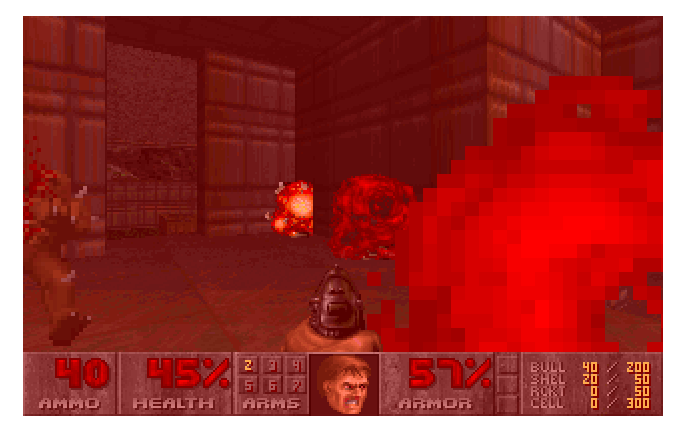
\includegraphics[scale=0.5]{./pics/doom}
  \caption{Application running Doom using js-dos}
  \label{fig:doom}
\end{figure}

\subsection{Module V.3}

The third and hopefully final, plan:

\begin{enumerate}
  \item Everything is a module
  \item Modules can \textit{invoke} modules
\end{enumerate}

A module only exposes a singular function:

\paragraph{Init} Returns a collection of modifications

\subsubsection{Tech Stack}

As mentioned in the previous section, the tech stack splits the application into
two, loosely coupled parts. The \textit{frontend} and \textit{backend}. This
architecture does facilitate the concept of an agnostic frontend. That is, if,
as is the case per the previous plan, all logic pertaining to the core is in the
\textit{frontend}, cannot the backend be anything, as long as it fulfills
\todo{List these criteria out}
certain criteria?
So that was a part of the new plan, avoid creating a \textit{backend}-module
system, similar to the \gls{rsms} mentioned previously. The functionality or
rather capability to extend the core application with modules written in Rust
exist, but would be a future core maintainers job. This would greatly simplify
the implementation of the core application, as a simplified \textit{backend}
could be created, only offering simple functionality, like access to the file
system. This plan would still keep the support for external JavaScript
libraries, not made with the application in mind, to be used, which also would
greatly reduce the development time.

\subsubsection{Tree Manipulation}

\todo{Mention how state and UI manipulation is equivalent to tree manipulation}

This restructure changes the way the view is render. Instead of the view being
re-rendered for each state-update, the view, or \gls{ui}-hierarchy, is only
\todo{Mention earlier how React was used/considered due to the "smart" re-rendering}
modified by modules. This modification is similar to the earlier state
modification, so a unified algorithm to solve this can be used. If there is an
easy way to translate a \gls{ui} modification to a state modification, and back
again. To solve this, instead of having a module return the actual
modifications, meaning, the updated core, a module returns a set of instructions
of what to do with the Core.
\todo{Add trivial module example, or something}

Using this as a module developer is quite abstract, so to facilitate development
of modules, a helper class was created, which \textit{translates} modifications
to instructions. These instructions can then be analyzed for possible
collisions. This solves the edge-case of a non-colliding modification of an
object in the state.

\begin{center}
  \lstinputlisting
   [ language=Haskell
   , caption={Module Type}
   , label=lst:moduleType
   ]{./code/module-example.hs}
\end{center}

As one can see in listing \ref{lst:moduleType}, a module only exposes its name,
and an \lstinline[language=haskell]{init} function, which takes the
\lstinline[language=haskell]{Core} \textit{ADT}, which is a representation of
the core application shown in listing \ref{lst:coreAdt}.

\begin{center}
  \lstinputlisting
   [ language=Haskell
   , caption={Module Unverified Type}
   , label=lst:moduleTypeUnverified
   ]{./code/module-unverified-example.ts}
\end{center}

This architecture also has the issue about verification of modules, but only on
functions, as simple fields can be validated using the
\lstinline[language=JavaScript]{typeof} operator. It is possible to do
\textit{some} verification on functions in TypeScript, but this is only a) Is it
a function, and b) does it have the correct amount of arguments. In this case,
one. Nothing about the typing of the function can be ascertained at runtime,
without explicitly invoking the function.

\begin{center}
  \lstinputlisting
    [ language=Haskell
    , caption={Core ADT}
    , label=lst:coreAdt
    ]{./code/module-example-core.hs}
\end{center}

In listing \ref{moduleEvent}, one can see the structure of an
\lstinline[language=Haskell]{Event} \textit{ADT}. This allows for modules to
pattern match on specific \lstinline[language=Haskell]{Event}s, and as in the
previous version, only react to specific \lstinline[language=Haskell]{Event}s.
What is different, is as shown in the \ref{lst:moduleCounter} listing, is that
each module registers an \lstinline[language=Haskell]{EventHandler} which is
\textit{only} invoked when the specific \lstinline[language=Haskell]{Event} it
is registered with, is called. This ensures a more direct form of
module-to-module communication, as a module can directly \textit{invoke} another
module. This changes the structure of the module architecture to go from one
wherein the core is a terminal object, to a more \textit{complicated} one, in
which module families can form.

\begin{center}
  \lstinputlisting
    [ language=Haskell
    , caption={Module Event Type}
    , label=lst:moduleEvent
    ]{./code/module-example-event.hs}
\end{center}

\begin{center}
  \lstinputlisting
    [ language=Haskell
    , caption={Module Counter Example}
    , label=lst:moduleCounter
    ]{./code/module-example-counter.hs}
\end{center}

\begin{center}
  \lstinputlisting
    [ language=Haskell
    , caption={Module Counter Example Event Handler}
    , label=lst:moduleEventHandler
    ]{./code/module-example-counter-handler.hs}
\end{center}

The module example shown in listing \ref{lst:moduleCounter} and
\ref{lst:moduleEventHandler}, is again, a simple counter example, where the
module registers a \lstinline[language=Haskell]{CoreModification}, changing the
UI-hierarchy, by adding a button which throws an
\lstinline[language=Haskell]{Event} that is handled by the
\lstinline[language=Haskell]{EventHandler} shown in
\ref{lst:moduleEventHandler}, which again, modifies the core by changing the
counter field with the value from the \lstinline[language=Haskell]{Event}.
